\documentclass{article}
\usepackage{graphicx}
%pages setting
\usepackage{geometry}
\geometry{a4paper, centering, scale = 0.8}

\title{COMSM0104-Web Technologies Report}
\author{Kehan Du, Shunyi Zhao}

\begin{document}

\maketitle

\section{Introduction}
\subsection{Project Introduction}
Our team is comprised of Kehan Du (mz19460) and Shunyi Zhao (vt19049). The
aim of our project is to construct the PC end official website of Deep KW
Innovation Factory.

~\\
\noindent
Deep KW Innovation Factory is the academic workshop of interdisciplinary 
at Huazhong University of Science and Technology, China. Since the establishment 
of Deep KW Innovation Factory in 2017, it has always upheld and practiced 
the concepts and methods of interdisciplinary, and insisted on exploring 
the question of social sciences by using natural science methods.

~\\
\noindent
The central goal of this version is to construct of the official website 
framework and the dynamic realization of key pages and complete the initial 
launch of the official website. This version is just used to practice the skills
of web technologies, and will not be used commercially. We have got the
permission to develop this website.

~\\
\noindent
Because of the dangerous circumstance, we use GitHub to work together.

\subsection{Development Method}
The following operations will instantly start the project:
\begin{itemize}
    \item git clone https://github.com/lele1307/DeepKW.git
    \item cd Server
    \item npm install
    \item npm run start
    \item cd project
    \item npm install
    \item npm run dev
\end{itemize}

\section{Technology Evaluation}
\subsection{Estimation of marks}
\begin{itemize}
    \item A for HTML
    \item A for CSS
    \item A for JS
    \item A for PNG
    \item B for SVG
    \item B for Server
    \item B for Database
    \item B for dynamic pages
    \item 12 for Depth (out of 20)
\end{itemize} 

\subsection{Client Side}
We chose a popular javascript framework, Vue.js (version 2.6.11), to 
develop these pages.
Modularity and componentization are important features of Vue,  
allowing us to build complex applications with small, independent, 
and usually reusable components. And these components convenient 
for later maintenance and upgrade of the official website. 
We use webpack and npm manage the packages based on node.js, and 
information about these packages is shown in package.json. Works are 
placed in folder named \textit{./src/components}. HTML, used as 
the template of every module, and CSS will control the layout 
and style of these modules.

\subsubsection{HTML}
HTML is an integral part of the Vue component demonstrated as \textless template\textgreater \space
tag. 
Vue.js uses an HTML-based template syntax that allows programmers to declaratively 
bind the rendered DOM to the underlying Vue instance’s data. The advantage of Vue 
is it compiles the templates into Virtual DOM render functions. Combined with the 
reactivity system, Vue is able to intelligently figure out the minimal number of 
components to re-render and apply the minimal amount of DOM manipulations when the 
app state changes.

~\\
\noindent
In our project, only one index.html document is used as the entrance, which is 
accessed through index.js.Other pages are all broken down into components, 
which are stitched together like building blocks.Compared with basic .html 
document, Vue's template HTML reduces the replication of many HTML statements. 
At the same time, the grammar in the Vue framework makes the data no longer 
nested in HTML statements, making the project itself more flexible.

~\\
\noindent
In this project, BaseNav.vue \textit{project/src/components/Common/BaseNav.vue}
is a good example. This is a common Navigation component, which uses list 
rendering to render the navigation name(data) into HTML, and completes 
the task with a brief HTML statement.

\begin{figure}[h]
    \centering
    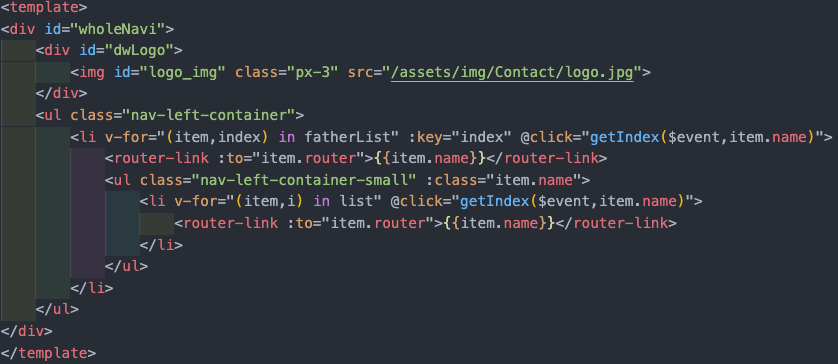
\includegraphics[width=13cm]{img/exp/html.png}
    \caption{The HTML codes written in BaseNav.vue}
    \label{}
\end{figure}
\subsubsection{CSS}
CSS is also an integral part of the Vue component demonstrated 
as \textless style\textgreater. The advantage is that the scope of CSS can be 
limited by adding the "scoped" attribute.

~\\
\noindent
Vue supports a variety of CSS, Less, Sass style expression mode, 
this project uses basic CSS for style editing. At the same time, 
we also carried out basic beautification of some HTML parts with 
the help of Bootstrap4. The use of Flexbox in the layout, 
this method effectively improves the website screen adaptability.

~\\
\noindent
Original CSS  can be reflected in groups.vue
\textit{project/src/components/About/groups.vue}. 
Finally achieving the 
predetermined goal of the design diagram.

\begin{figure}[h]
    \centering
    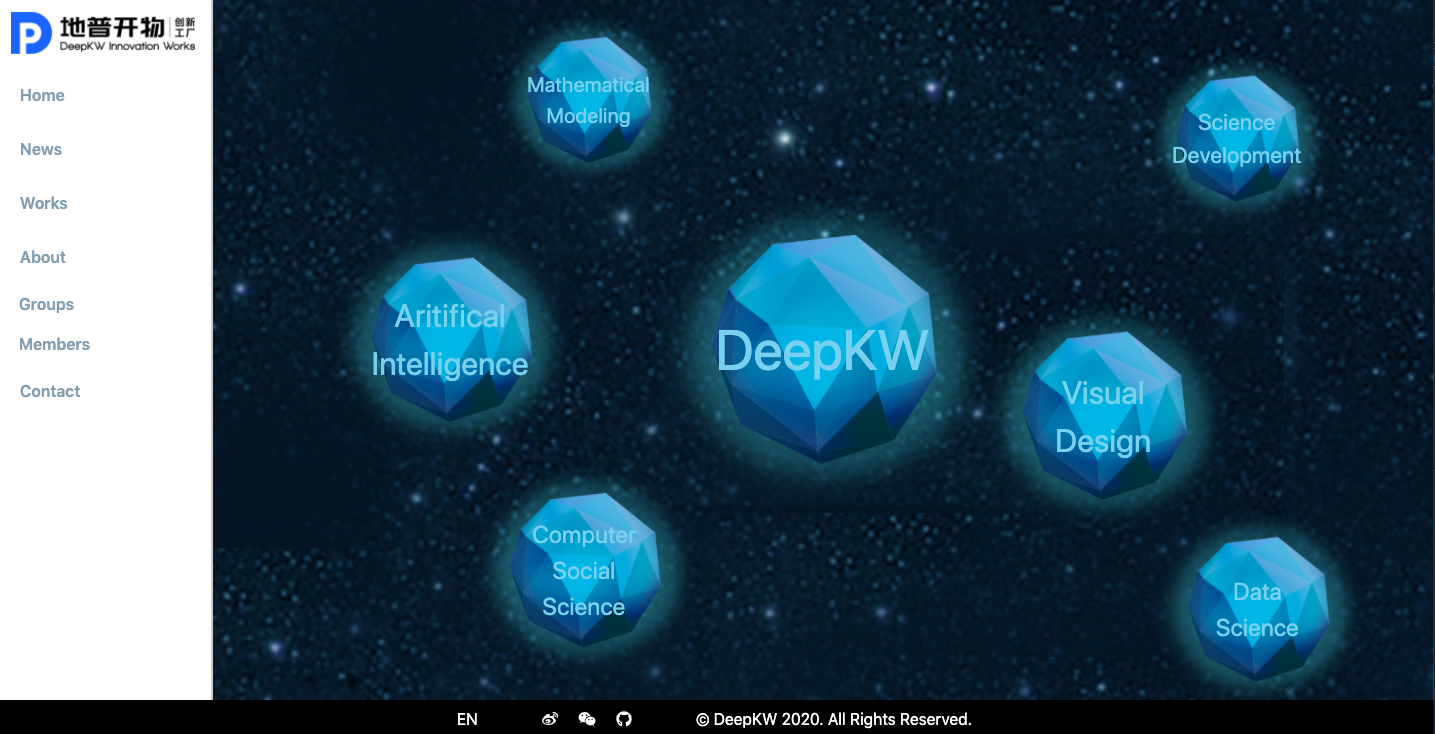
\includegraphics[width=10cm]{img/exp/css.png}
    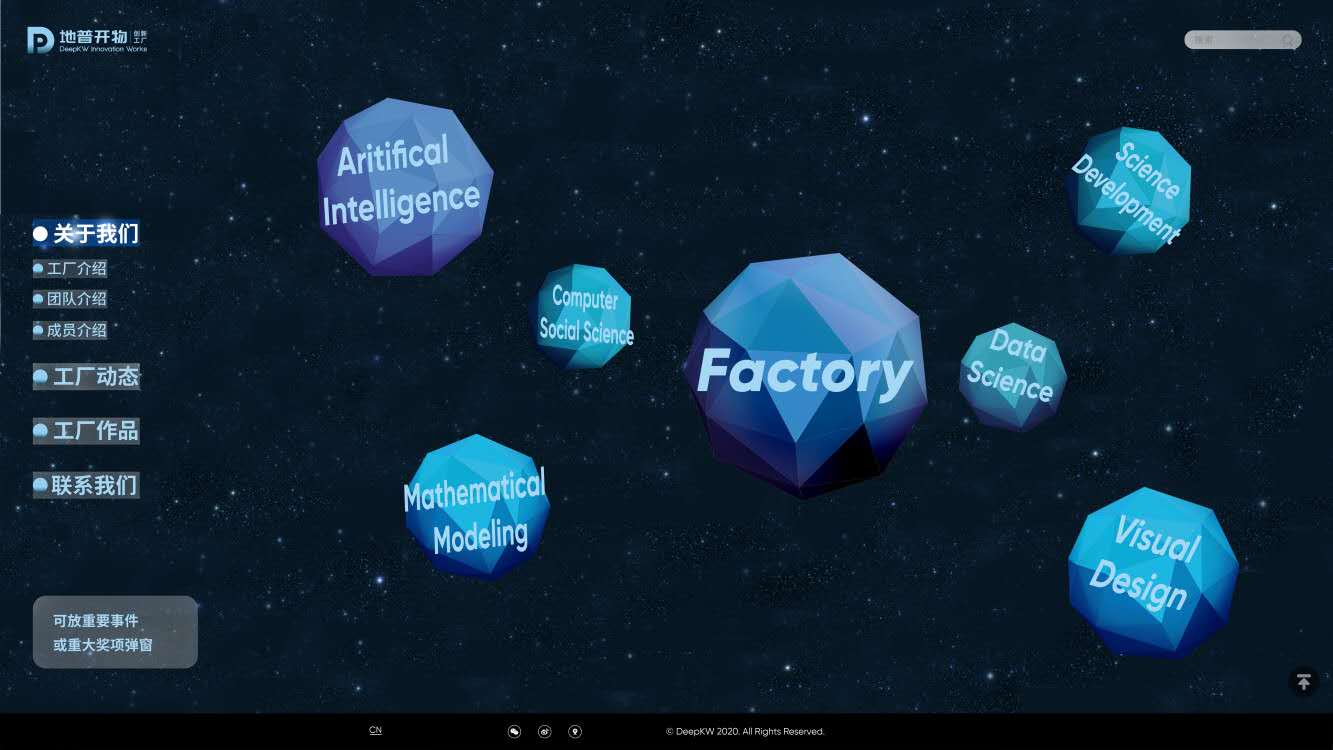
\includegraphics[width=10cm]{img/05.jpg}
    \caption{Design sketches and final layout}
    \label{}
\end{figure}

\subsubsection{JavaScript}
The embodiment of Javascript on the client-side is the Vue.js framework. 
From the structural point of view, index.js is used as the entrance 
into the program, router.js is the route deployment of the subpage 
of the website, and other specific js methods are written in 
the \textless script\textgreater\space tag of each component.

~\\
\noindent
There are some examples of specific JS methods:
\begin{itemize}
    \item The pop-up effect of the About-Group page
    \item Hide and show the title of the navigation bar subset
    \item News / Works pages read data from the database in the light of requirements
\end{itemize}

~\\
\noindent
In addition, we used the Webpack packaging tool to modularize and 
unify a large number of CSS, JS and other dependent files. To a certain 
extent, the page loading capacity has been optimized.

~\\
\noindent
The entire Vue project does not rely on Vue CLI scaffolding, 
and the project configuration files are all original.

\subsubsection{PNG}
Some images used in this project are drawn with GIMP 2. One of the examples,
textit{table.png} which is ued in \textit{Contact.vue}, is shown below in 
Figure \ref{fig: figure2}.

\begin{figure}[h]
    \centering
    
\includegraphics{img/sectionPNG/table2.png}
    
\includegraphics{img/sectionPNG/table1.png}
    \caption{Left: the image after adding three text objects. 
    Right: add three rectangles with 48.0 opaqueness.}
    \label{fig: figure2}
\end{figure}

~\\
\noindent
Some background and unimportant images are cited from the Internet.

\noindent
Firstly, we added three text objects into a $ 300 \times 400 $ file, and then 
typed in some useful information. Then the coverages of these text objects are
combined to fix the positions of them. The result of this stage is shown in the 
left image of Figure \ref{fig: figure2}. And then, three rectangular layers are 
added, the result is shown in the right image of Figure \ref{fig: figure2}. 



\subsubsection{SVG}
We tried to use Inkscape as a tool for original SVG design.
\begin{itemize}
    \item The arrow shape mainly reflected in Contact page \textit{project/src/assets/img/Contact/arrow.svg}.
    \item LOGO  of \textless title\textgreater\space tag is converted to ico format via svg.
\end{itemize} 

\begin{figure}[h]
    \centering
    
\includegraphics[width=4cm]{img/exp/svg1.png}
    \caption{Logo of title}
    \label{}
\end{figure}

~\\
\noindent
In addition to the original SVG, the project also references the 
font-awsome icon font library. This font library can provide 
scalable vector icons. Its scalability can better adapt to the page size.
\begin{figure}[h]
    \centering
    
\includegraphics[width=10cm]{img/exp/svg.png}
    \caption{Svg examples}
    \label{}
\end{figure}

\subsection{Sever Side}
\subsubsection{Server}
The development of Sever is also in node.js. We use \textit{express} as the 
server framework. The main works of Server is placed in the path (Server/routes),
including three .js file. The file submit.js is used to accept the information 
sent by the webpage Contact. This file use the function called get() to accept and 
send the response to the webpage. With the prepared statement of sql, this file 
could use a query to store these information into the database. Because the primary
key of the table used in this file is not set to a auto-increment attribute, this
file will also use a select query to count the number of rows in this table, to 
calculate the number which should be inserted.

The port number used in the sever side is set to 3000. Because some rules ban the 
direct communication between the client side and the server side, we use a feature
of axios to send the information. This proxy is set in the file
\textit{./project/webpack.config.js}.
\subsubsection{Database}
We choose \textit{sqlite3} to manage our databases. 
We use three tables, including candidata, news and work in this project.

~\\
\noindent
The table candidata is used to store the data submitted by users. This table
has six attributes, including id (primary key), name, gender, country, university
and info. The table work has five attributes, including id, type, subject, title 
and content.

~\\
\noindent
All queries used by the server files is written in prepared statements. We use
these queries to get information from database and insert a new row into it. We
also use some callback functions to ensure the programmes get the information 
in order.



\subsubsection{Dynamic Page}
A good example of dynamic page in our project is the \textit{Works} page.
We develop a method called getAll() in the file
\textit{project/src/components/Works/Selecter.vue}. This method is also used in the 
created part of Vue, which could get the data of all the works stored in databases
when this webpage is initialized. The layout of this page is shown below in 
Figure ~\ref{fig: figure5}.

\begin{figure}[h]
    \centering
    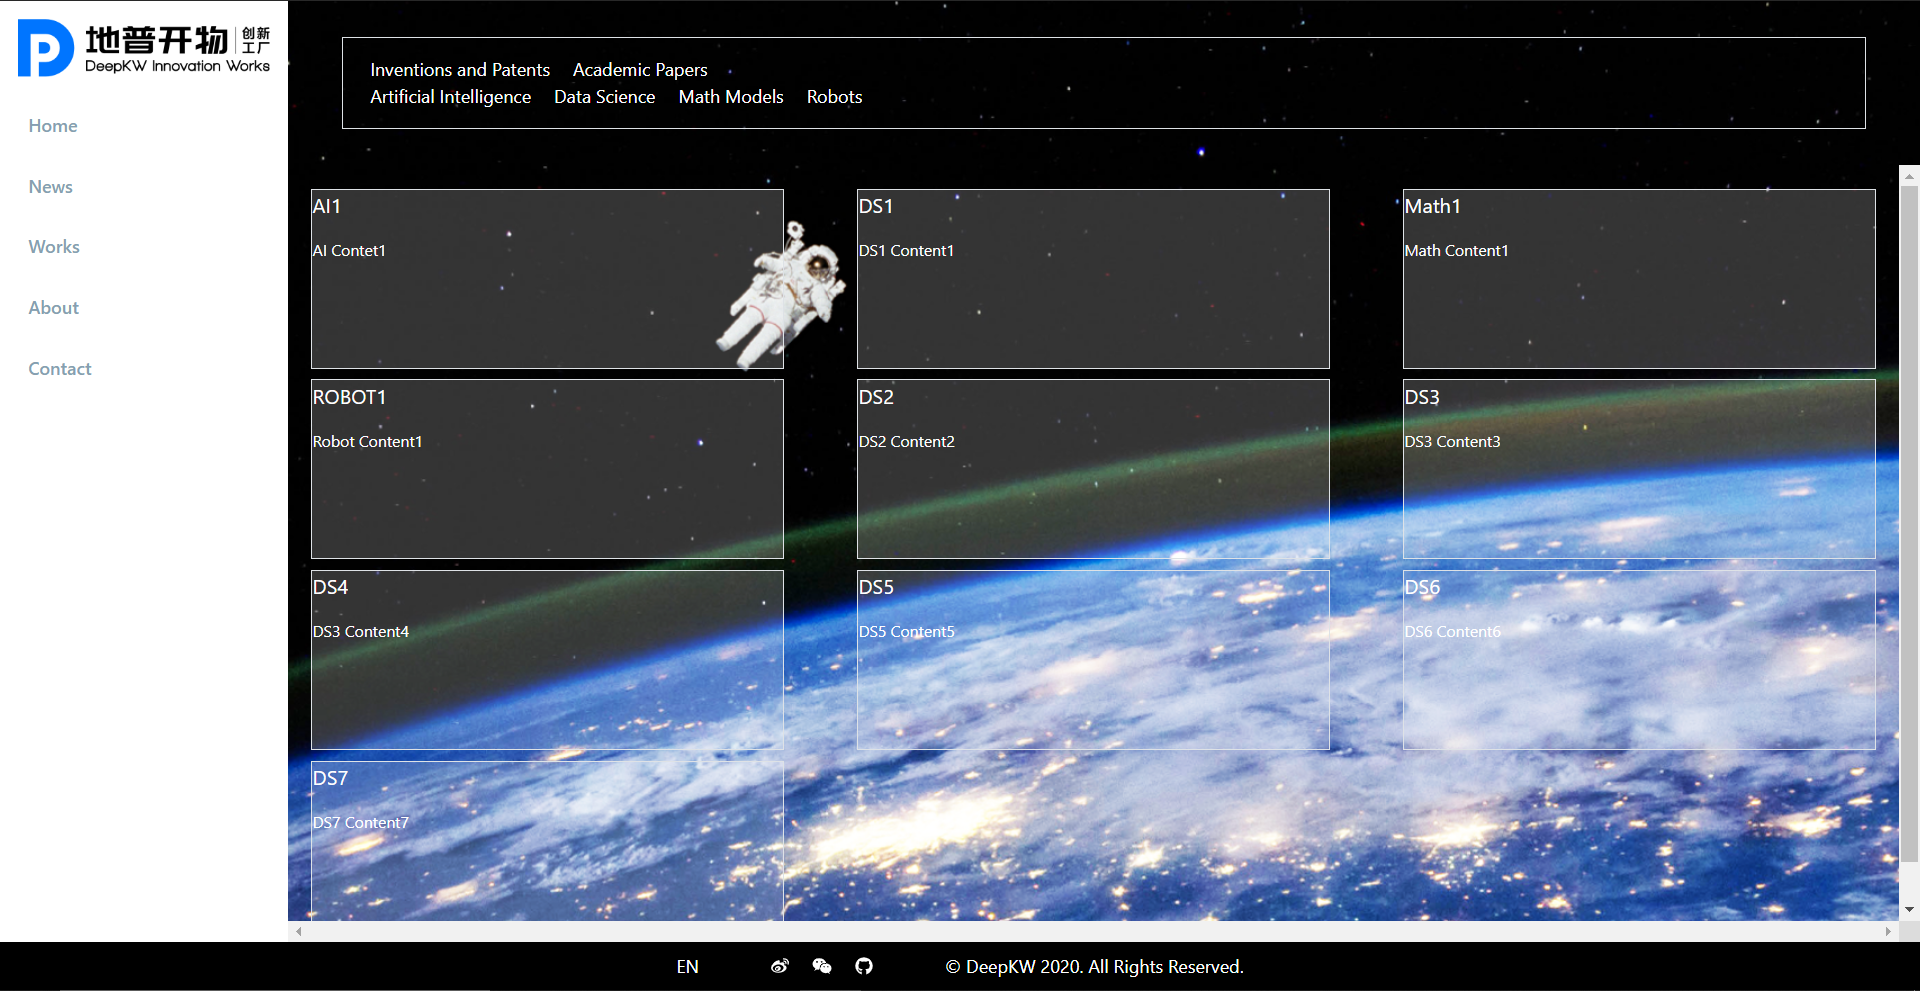
\includegraphics[height=4cm]{img/sectionPNG/Works1.png}
    \caption{The layout of Works page when open it}
    \label{fig: figure5}
\end{figure}

~\\
\noindent
Users could choose a type and a subject in the selection region in this page.
If a user choose more than one option, only the first type and the first subject
will be used to get information from server. If an option is chosen, the background
of this option bacome white. The works of academic papers about data science is shown
in Figure ~\ref{fig: figure6}.

\begin{figure}[h]
    \centering
    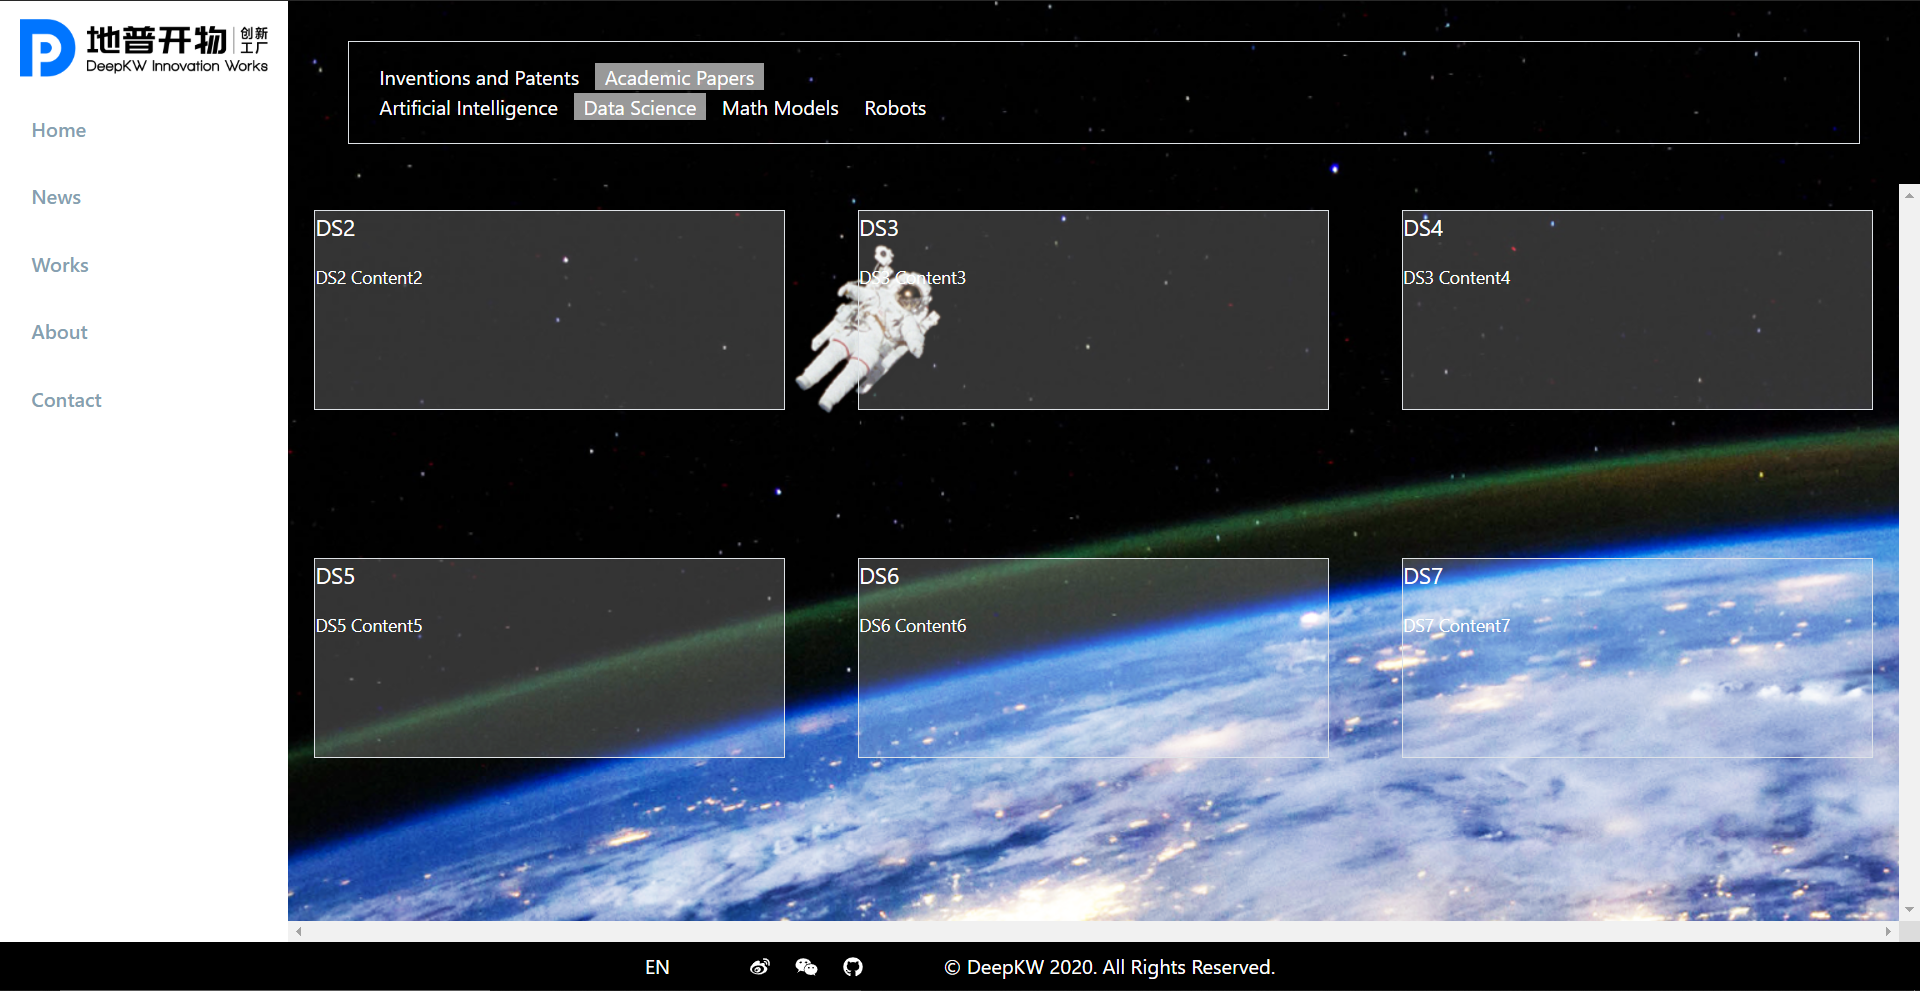
\includegraphics[height=4cm]{img/sectionPNG/Works2.png}
    \caption{Works of academic papers about data science}
    \label{fig: figure6}
\end{figure}

~\\
\noindent
A scroll bar is used to show more works.

\section{Evaluation}
\subsection{Deficiencies}
The construction of the website is basically completed, including 
the communication between the client and the server, and the 
configuration of the database. However, some styles and functions 
on the sub-webpage are still unfinished. For example, the About-Member
page is just the basic layout, with simple JS interaction methods, 
but the formal style has not been completed yet and needs further improvement.

This website is suitable for PCs, but we have not fully considered the issues
of screen adaptation and browser compatibility.
\subsection{Teamwork}
Our two-person team mainly uses Git for version control and 
GitHub for code merging and storage. Only in the circumstance 
of online communication, this tool greatly improves work 
efficiency. In the early stage of development, we agreed 
to use the Vue.js framework. At the same time, we have 
been learning by ourselves and helping each other. 
Although the final product still has a gap to launching, 
the first Web development experience is still impressive for us.
    
\end{document}
